%- HandOut Flag ----------------------
\makeatletter
\@ifundefined{ifHandout}{%
  \expandafter\newif\csname ifHandout\endcsname
}{}
\makeatother

%- D0cum3nt ----------------------------------------------------------------------------------------------
\documentclass[beamer,10pt]{standalone}   
%\documentclass[beamer,10pt,handout]{standalone}  \Handouttrue  

\ifHandout
	\setbeameroption{show notes} %print notes   
\fi

	
%- Packages ----------------------------------------------------------------------------------------------
\usepackage{custom-style}
\usepackage{math}



%--Beamer Style-----------------------------------------------------------------------------------------------
\usetheme{toninus}
\usepackage{animate}
\usetikzlibrary{positioning, arrows}
\usetikzlibrary{shapes}


%- Bibliography (Biber) ----------------------------------------------------------------------------------
\usepackage[backend=biber,style=alphabetic,maxnames=2]{biblatex}
\bibliography{bibfile.bib}

%===========================================================%
\begin{document}
%===========================================================% 
\checkpoint

%- . - . - . - . - . - . - . - . - . - . - . - . - . - . - . - . - . - . - . - . - . - . - . - .%	
\subsection{Regular reduction} 
%- . - . - . - . - . - . - . - . - . - . - . - . - . - . - . - . - . - . - . - . - . - . - . - .%	
\begin{frame}{Regular reduction in symplectic geometry}

	\textbf{\color{UniGreen}Symplectic reduction:}~~
	\\ 
	{\it \small
	Procedure associating to any (suitably regular) pair of \textbf{symplectic manifold} and \textbf{Hamiltonian action} another symplectic manifold of smaller dimension.}
	\vfill

	\pause
	
	\begin{center}
		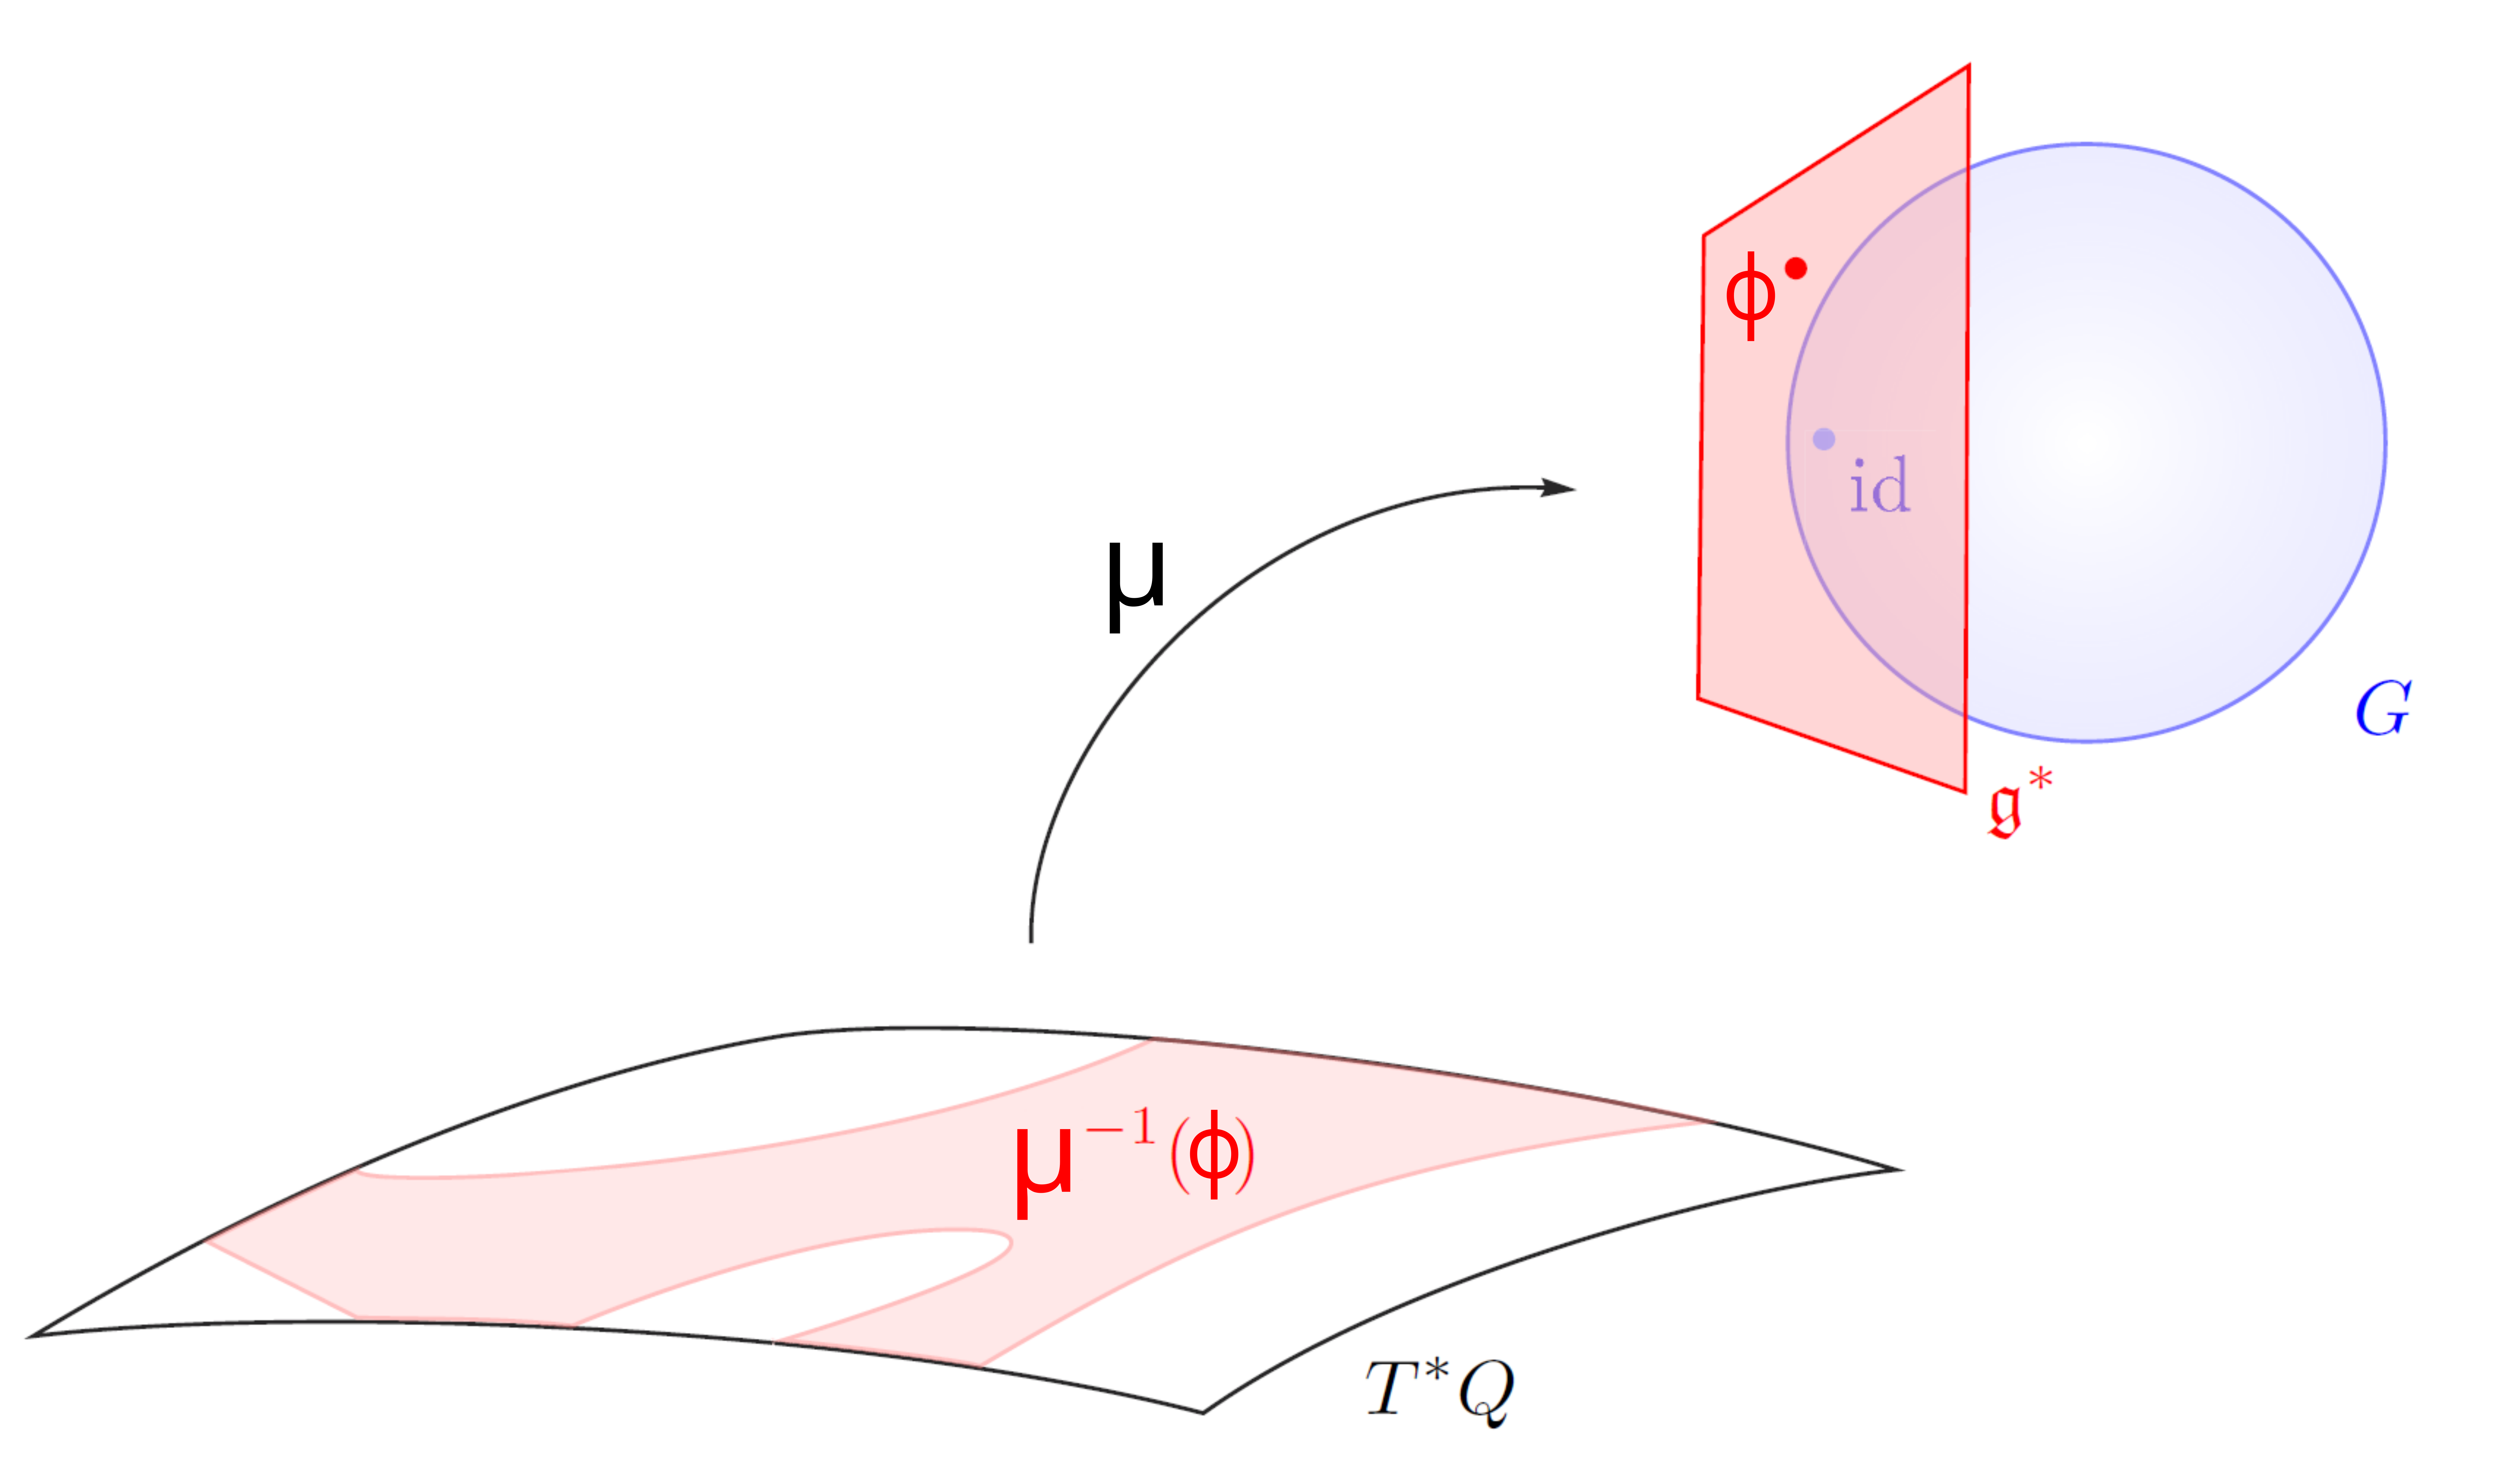
\includegraphics[width=.5\textwidth]{Pictures/Reduction}	
	\end{center}
	
	\textbf{\color{UniGreen}In mechanics:}~~
				\\
			{\it \small
				it embodies the process of restricting the dynamics of the system to the level sets of the conserved quantities pertaining to the symmetry group.		
			}
			\\[.2em]
			\color{gray}\small( e.g. restricting to studying a point-like particle in a central potential by studying it in radial coordinates)

\end{frame}
\note[itemize]{
	\item  \emph{(Credits to \href{https://math.gmu.edu/~cblacke/}{Casey Blacker} for the notes and to \href{https://arxiv.org/abs/1206.3302}{Christian Lessig} for the picture. See acknowledgements.}
	\item  In classical mechanics symmetry reduction plays an important role. Mathematically, this is usually phrased in terms of Marsden-Weinstein reduction
	\item {Symplectic Reduction} takes two inputs:
	\\ 1. Hamiltonian $G$-space $(M,\omega,{\color{orange}G},{\color{blue}\mu})$
	\\ 2. parameter ${\color{blue}\phi}\in\g^*$
	\item The \emph{reduced space} is $M_\phi:={\color{blue}\mu^{-1}(\phi)}{\color{orange}/G_\phi}$.
	\item (Marsden--Weinstein '74, Meyer '73) THM:\\
		If $\mu^{-1}(\phi)\subset M$ is smooth and $G_\phi\curvearrowright \mu^{-1}(\phi)$ is free and proper, then there is a \textbf{unique symplectic form} $\omega_\phi\in\Omega^2(M_\phi)$ such that $\pi^*\omega_\phi = i^*\omega$.



	\item Heuristic Approach to Reduction:
	\\1. describe $G\curvearrowright M$ in terms of $\omega$ 	\hspace{1cm}
	({\color{green}moment map $\mu$})
	\\2. identify a distinguished reduced space \hspace{1cm}
	({\color{green}reduction at $\mu=0$})
	\\3. use the ambiguity in 1.\ to obtain a family of reduced spaces \hspace{1cm}
	({\color{green}reduction at $\mu-\phi=0$, i.e.\ reduction at $\mu=\phi$}
	\\
	{\tiny Note: If $G_\phi\neq G$, then $\mu-\phi:M\to\g^*$ is not a moment map for either $G\curvearrowright M$ or $G_\phi\curvearrowright M$.}
	
}
%- . - . - . - . - . - . - . - . - . - . - . - . - . - . - . - . - . - . - . - . - . - . - . - .%	


 
%- . - . - . - . - . - . - . - . - . - . - . - . - . - . - . - . - . - . - . - . - . - . - . - .%
\begin{frame}[fragile]{Marsden-Weinstein-Meyer reduction}
	Consider: \quad $(M,\omega)$ symplectic,\quad $\theta:G\curvearrowright M$ $G$-action,\quad $\underline{\cdot}:\mathfrak{g}\to \mathfrak{X}(M)$ $\g$-action.
	\vfill\pause

	\begin{defblock}[Equivariant moment map]
		Smooth map $\quad\mu:M\to \mathfrak{g}^\ast\quad$ such that:
		
		\quad {\it i)} $\d\langle \mu,\xi\rangle = -\iota_{\underline{\xi}}\omega$,
		\qquad {\it ii)}  $\mu \circ \theta_g = Ad_g^\ast \circ \mu$,
		\qquad $\forall \xi \in \mathfrak{g},~ \forall g \in G$.
	\end{defblock}
	\vfill\pause

	\begin{thmblock}[Marsden-Weinstein reduction \cite{MarsdenWeinstein74}]
		\vspace{-.4em}\hspace{-1em}
		\begin{tabular}{l p{14cm}}
			Given: &   $\mu:M\to \mathfrak{g}^*$ equivariant moment map for $\color{orange}G\curvearrowright M$ $G$
			\\[.2em]
			Assume: & ${\color{blue}\phi} \in \mathfrak{g}^*$ regular value of $\mu$ 
			\qquad\quad \footnotesize \textcolor{gray}{($\Rightarrow$ $\mu^{-1}(\phi)\hookrightarrow M$ smooth embedding)}
			\\
			& $G_\phi\curvearrowright \mu^{-1}(\phi)$ free and proper
			\quad \footnotesize \textcolor{gray}{($\Rightarrow$ $\mu^{-1}(\phi)/G_\phi$ smooth manifold)}
			\\[.4em]
			Then: & \textbf{$\exists!$ symplectic structure} $\omega_\phi$ in $M_\phi:={\color{blue}\mu^{-1}(\phi)}{\color{orange}/G_\phi}$ \\
			& s.t. $\pi^\ast \omega_\phi = j^\ast \omega$ 
			\qquad {\footnotesize with $j:\mu^{-1}(\phi) \hookrightarrow M$ and $\pi:\mu^{-1}(\phi)\twoheadrightarrow M_\mu$}
		\end{tabular}
		\vspace{-.4em}
	\end{thmblock}
	%
	\vfill
	\begin{center}
	\begin{tikzpicture}[scale=2]
		\node[blue] (A) at (0,0) {$\mu^{-1}(\phi)$};
		\node[gray] (A1) at (0,.3) {$i^*\omega$};
		\node[gray] (A2) at (-.6,0) {$\pi^*\omega_\phi$};
		\node[blue] (B) at (1,0) {$M$};
		\node[gray] (B1) at (1,.3) {$\omega$};
		\node[orange] (C) at (0,-.8) {$M_\phi$};
		\node[gray] (C2) at (-.6,-.8) {$\omega_\phi$};

		\path[right hook->,blue] (A) edge node[above] {$i$} (B);
		\path[orange,->] (A) edge node[left] {$\pi$} (C);
		\begin{scope}[xshift=-1.8cm]
			\node[blue] at (0,0) {\small restrict to $\{\mu=\phi\}$};
			\node[orange] at (.15,-.4) {\small quotient by $G_\phi$};
		\end{scope}
	\end{tikzpicture}
	\end{center}


\end{frame}
\note[itemize]{
 \item 
	Let $(M,\omega)$ symplectic, $G\circlearrowright M$ be a Lie group action\pause and $\mu:M\to \mathfrak g^*$ such that: 
	\item  $\mu$ is a momentum, i.e. the infinitesimal action $\xi\mapsto \underline\xi:\mathfrak g\to \mathfrak X(M)$ of $G$ satisfies $X_{\langle\mu,\xi\rangle}=\underline \xi$. 
	\item $\mu$ is $G$-equivariant, i.e. $\mu(gm)=Ad^*_g\mu(m)$ 
	\item Then $\exists!$ symplectic form $\omega_r$ on $M_r=\frac{\mu^{-1}(0)}{G}$ such that $\pi^*\omega_r=i^*\omega$.
%% https://q.uiver.app/#q=WzAsMyxbMCwwLCJNIl0sWzMsMCwiXFxtdV57LTF9KDApIl0sWzYsMCwiTV9yIl0sWzEsMCwiaVxcXFwgXFxzdWJzdGFja3tpbmNsdXNpb25+b2Z+c3Vic3BhY2V9IiwyLHsic3R5bGUiOnsidGFpbCI6eyJuYW1lIjoiaG9vayIsInNpZGUiOiJib3R0b20ifX19XSxbMSwyLCJcXHBpXFxcXCBcXHN1YnN0YWNre3F1b3RpZW50fmJ5fnJlbGF0aW9ufSJdXQ==
%\[\begin{tikzcd}
%	M &&& {\mu^{-1}(0)} &&& {M_r}
%	\arrow["\begin{array}{c} i\\ \substack{inclusion~of~subspace} \end{array}"', hook', from=1-4, to=1-1]
%	\arrow["\begin{array}{c} \pi\\ \substack{quotient~by~relation} \end{array}", two heads, from=1-4, to=1-7]
%\end{tikzcd}\]
	\item 	The action of $G$ on $\mu^{-1}(0)$ is free and proper $\Rightarrow$ $0$ is reg. val. of $\mu$


}
%- . - . - . - . - . - . - . - . - . - . - . - . - . - . - . - . - . - . - . - . - . - . - . - .%


 


%- . - . - . - . - . - . - . - . - . - . - . - . - . - . - . - . - . - . - . - . - . - . - . - .%
\subsection{Singular reduction}
\begin{frame}{Symplectic singular reduction schemes}
	\begin{block}{The gist of singular reduction}
		 \begin{itemize}
			 \item[-] when $\mu$ is singular (i.e. $\mu^{-1}(0)$ is not a mfd.), the (geometrically) reduced space may not exist.
			 \item[-] a \emph{singular reduction scheme} is a procedure to construct a "reduced" algebra of observable out of the given data
			 \item[-] such that it corresponds to the algebra of observable of the reduced manifold in the regular case.
		 \end{itemize}
	\end{block}
	 %
	 \pause
	 \vfill
	 %
	\begin{thmblock}[Sniatycki-Weinstein reduction \cite{SniatyckiWeinstein83}]
		\vspace{-.4em}\hspace{-1em}
		\begin{tabular}{l p{14cm}}
			Given: & $(M,\omega)$ symplectic
			\\
			& $G\curvearrowright M$ symplectic with equivariant momap. $\mu:M\to \mathfrak{g}^*$
			\\[.4em]
			Then: & 
			$\displaystyle \left[\sfrac{C^\infty(M)}{I_\mu}\right]^G$
			admits a Poisson algebra structure 
			\footnote{$I_\mu$ = associative ideal generated by $\check{\mu}(\g)$ with $\check{\mu}(\xi):=\langle\mu,\xi\rangle$ the comomentum map.}			
			\\
			& it agrees with the M--W reduction in the regular case.		
		\end{tabular}
		\vspace{-.4em}
	\end{thmblock}
 \end{frame}
\note[itemize]{
 \item Let $(M,\omega,G,\mu)$ be a symplectic Hamiltonian $G$-space.
 \item The \emph{momentum ideal} is the associative ideal $I_\mu\subset C^\infty(M)$ generated by the momenta $\mu_{\xi}$ for any $\xi\in \mathfrak{g}$.
		Namely
		\[
			I_\mu 
			= 
			\Big\langle \mu_\xi \Big\rangle_{\xi \in \mathfrak{g}}^{\text{\tiny asso.}} 
			=
			\left\{
				\left.
					\sum_{i=1}^n f_i ~ \mu_{\xi_i}
				\right|~
					f_i \in C^\infty(M),~ \xi_i\in \mathfrak{g},~  1 \leq i \leq n
			\right\}
		\]

 \item The \emph{\'Sniatycki--Weinstein reduction} is the Poisson algebra
		\[
			\left(C^\infty(M)/I_\mu\right)^G.
		\]


}
%- . - . - . - . - . - . - . - . - . - . - . - . - . - . - . - . - . - . - . - . - . - . - . - .%	











%- . - . - . - . - . - . - . - . - . - . - . - . - . - . - . - . - . - . - . - . - . - . - . - .%
\subsection{Constraints Algebras}
\begin{frame}[fragile]{Attempting algebraic reduction naively}
When the action is not 'free and proper', we can try to mimic this directly using the function algebras:
% https://q.uiver.app/#q=WzAsNixbMCwwLCJNIl0sWzEsMCwiXFxtdV57LTF9KDApPVMiXSxbMywwLCJNX3IiXSxbMCwxLCJDXlxcaW5mdHkoTSkiXSxbMSwxLCJDXntcXGluZnR5fShTKT1cXGZyYWN7Q157XFxpbmZ0eX0oTSl9e0lfe1N9fSJdLFszLDEsIkNee1xcaW5mdHl9KE1fcik9Q15cXGluZnR5KFMpXkciXSxbMSwyLCJcXHN1YnN0YWNre3F1b3RpZW50fSIsMCx7InN0eWxlIjp7ImhlYWQiOnsibmFtZSI6ImVwaSJ9fX1dLFszLDQsIlxcc3Vic3RhY2t7cXVvdGllbnR9IiwwLHsic3R5bGUiOnsiaGVhZCI6eyJuYW1lIjoiZXBpIn19fV0sWzAsMSwiXFxzdWJzdGFja3tyZXN0cmljdGlvbn0iLDAseyJzdHlsZSI6eyJib2R5Ijp7Im5hbWUiOiJzcXVpZ2dseSJ9fX1dLFs0LDUsIlxcc3Vic3RhY2t7cmVzdHJpY3Rpb259IiwwLHsic3R5bGUiOnsiYm9keSI6eyJuYW1lIjoic3F1aWdnbHkifX19XV0=
\[\begin{tikzcd}
	M & {\mu^{-1}(0)=S} && {M_r} \\
	{C^\infty(M)} & {C^{\infty}(S):=\frac{C^{\infty}(M)}{I_{S}}} && {C^{\infty}(M_r)=C^\infty(S)^G}
	\arrow["{\substack{restriction}}", squiggly, from=1-1, to=1-2]
	\arrow["{\substack{quotient}}", two heads, from=1-2, to=1-4]
	\arrow["{\substack{quotient}}", two heads, from=2-1, to=2-2]
	\arrow["{\substack{restriction}}", squiggly, from=2-2, to=2-4]
\end{tikzcd}\]

where $I_S=\{f\in C^{\infty}(M)~|~f|_S=0\}$.
\pause 
\vfill
Equivalently:

% https://q.uiver.app/#q=WzAsMyxbMCwwLCJDXlxcaW5mdHkoTSkiXSxbMiwwLCJOX1M9XFx7Zn58fiBmXFxpbiBDXlxcaW5mdHkoTSl8X1N+fkdcXG1hdGhybXstaW52YXJpYW50fVxcfSJdLFs0LDAsIlxcZnJhY3tOX1N9e0lfU30iXSxbMCwxLCJcXHN1YnN0YWNre3Jlc3RyaWN0aW9ufSIsMCx7InN0eWxlIjp7ImJvZHkiOnsibmFtZSI6InNxdWlnZ2x5In19fV0sWzEsMiwiXFxzdWJzdGFja3txdW90aWVudH0iLDAseyJzdHlsZSI6eyJoZWFkIjp7Im5hbWUiOiJlcGkifX19XV0=
\[\small\begin{tikzcd}
	{C^\infty(M)} && {N_S=\{f~|~ f\in C^\infty(M)|_S~~G\mathrm{-invariant}\}} && {\frac{N_S}{I_S}}
	\arrow["{\substack{restriction}}", squiggly, from=1-1, to=1-3]
	\arrow["{\substack{quotient}}", two heads, from=1-3, to=1-5]
\end{tikzcd}\]
\pause
\vfill

\begin{alertblock}{Problem}
	$C^\infty(S)^G=\frac{N_S}{I_S}$ is not a Poisson algebra in general.
\end{alertblock}
(when constraints not first class, cf. Dirac reduction)
\end{frame}
\note[itemize]{
	\item \emph{(Credits to \href{https://www.ryvkin.eu/}{Leonid Ryvkin} for the tex code of this slide.)}
}
%- . - . - . - . - . - . - . - . - . - . - . - . - . - . - . - . - . - . - . - . - . - . - . - .%



%- . - . - . - . - . - . - . - . - . - . - . - . - . - . - . - . - . - . - . - . - . - . - . - .%
\begin{frame}{Constraint Algebras} 
	\begin{block}{Idea:}
	    \begin{itemize}[noitemsep,topsep=0pt,parsep=0pt,partopsep=0pt]
			\item[-] Both regular/geometric and singular/algebraic reduction are 2-steps procedures (1. restrict 2. quotient).
			\item[-] Let's work in a category where all data needed for the reduction are bundled together in a suitable categorical objects. {\tiny (To avoid pathologies arising from these steps)}
	    \end{itemize}
	\end{block}
	\pause
	\vfill
	\begin{defblock}[Constraint algebra triples \cite{Dippell2023}]
		A (strong embedded) constraint algebra $\mathcal A$ is given by a triple $(\mathcal A_T, \mathcal A_N, \mathcal A_0)$, where
		\begin{itemize}[noitemsep,topsep=0pt,parsep=0pt,partopsep=0pt]
			\item[•] $\mathcal A_T$ is an algebra \emph{("total space")}
			\item[•] $\mathcal A_N\subset \mathcal A_T$ a subalgebra  \emph{("normal space")}
			\item[•] $\mathcal A_0\subset \mathcal A_N$ a two-sided ideal in $\mathcal A_T$ \emph{("zero space")}
		\end{itemize}
	\end{defblock}
	\vfill
	\pause
	\begin{exblock}
		Let $S$ be a closed set. Algebraically, we describe $C^\infty(S)$ by $\frac{C^\infty(M)}{I_S}$.
		\\ 
		We can think of it as the constraint triple:
		$$
			\mathcal A=(\mathcal A_T,\mathcal A_N,\mathcal A_0)=(C^\infty(M),C^\infty(M), I_S)
		$$
	\end{exblock}

\end{frame}
\note[itemize]{
	\item  triples of the type (algebra , subalgebra, ideal).
	\item After \cite{Dippell2023} we call such triples { \bf constraint triples} and their parts \emph{total space, normal space, zero space}.
	\item It is a (strong) constraint algebra if $\mathcal A_0\subset \mathcal A_N\subset \mathcal A_T$ subalgebras and $\mathcal A_0\subset \mathcal A_T$ ideal.
}
%- . - . - . - . - . - . - . - . - . - . - . - . - . - . - . - . - . - . - . - . - . - . - . - .%


%- . - . - . - . - . - . - . - . - . - . - . - . - . - . - . - . - . - . - . - . - . - . - . - .%
\begin{frame}{A plethora of approaches to singular reduction}
 	Many singular reduction schemes adhere to this pattern!
 	\vfill
 	\pause
\begin{table}[]
	\begin{tabular}{l|l|l||l}
		algebra $\mathcal{A}_T$ & subalgebra $\mathcal{A}_N$ & ideal $\mathcal{A}_0$ & comment \\
		\hline
		
		$C^\infty(M)$&      $N_S$     &   $I_S$   &  $\substack{S=\mu^{-1}(0),~ I_S=\{f~|~f|_S=0\}}$ \\
			&&&  $\substack{N_S= \{ f | gf-f\in I_S \forall g\in G\}}$ \\
	& & & \color{red} not Poisson \\ 
	\hline	\pause
	$C^\infty(M)$&   $F_S$         &   $I_S$   &  $\substack{F_S=\{f~|~\{f,I_S\}\subset I_S\}}$ \\
	& & & \color{red} if $I_S\subset F_S$\\
	\hline \pause
	
	$C^\infty(M)$&   $C^\infty(M)^G$         &   $(I_S)^G$   &  $\substack{C^\infty(M)^G=\{f~|~gf=f\forall g\in G\}}$ \\
	\hline \pause
		$C^\infty(M)$&   $C^\infty(M)^G$         &   $(I_\mu)^G$   & $\substack{I_\mu=\{\sum_{i=1}^k f_i\langle \mu,\xi_i\rangle|~f_i\in C^\infty(M), \xi_i\in \mathfrak g\}}$\\
		\hline \pause
	$C^\infty(M)$&      $N_\mu$     &   $I_\mu$   & $\substack{N_\mu= \{ f | gf-f\in I_\mu \forall g\in G\}}$ \footnote{When $G$ connected $N_\mu=N(I_\mu):=\{f~|~\{f,I_\mu\}\subset I_\mu\}$.}\\
	\hline 
		
	\end{tabular}\pause
\end{table}
	\vfill
	{\bf Remarks }names in order: 'naive' , Dirac, Sniatycki, Arms-Cushman-Gotay, Sniatycki-Weinstein.

\end{frame}
\note[itemize]{
	\item \emph{(Credits to \href{https://www.ryvkin.eu/}{Leonid Ryvkin} for the tex code of this slide.)}
}
%- . - . - . - . - . - . - . - . - . - . - . - . - . - . - . - . - . - . - . - . - . - . - . - .%


%- . - . - . - . - . - . - . - . - . - . - . - . - . - . - . - . - . - . - . - . - . - . - . - .%
\begin{frame}{Constraint Gerstenhaber-Modules}

%
\begin{defblock}[Constraint Gerstenhaber algebra {(\cite[Def. 2.25]{dippelkern})}]
	A constraint algebra $G=\triple{G}$ equipped with a constraint bilinear map
	\begin{displaymath}
		\{ \cdot, \cdot \} \colon G[1] \otimes G[1] \to G[1]
	\end{displaymath}
	such that $G_\Total$ is a Gerstenhaber algebra. 
\end{defblock}
\pause\vfill
%

 \begin{remblock}[$G$ can be seen as a triple of Gerstenhaber subalgebras]\label{rk:constraintgerst-as-triple}
	 $G_\Null \subseteq G_\Wobs \subseteq (G_\Total, \wedge,\lbrace\cdot,\cdot\rbrace)$ such that $G_\Null$ is a Gerstenhaber ideal in $G_\Wobs$. 
\end{remblock}
\pause\vfill
%

\begin{defblock}[Constraint Gerstenhaber module]\label{def:constraintgerstmodule}
	A constraint vector space $V=\triple{V}$ endowed with a constraint Gerstenhaber algebra structure on the space $G \oplus V^\rev$ such that the multiplication and the bracket are trivial when restricted to $V^\rev$.
\end{defblock}
\vfill

\end{frame}
\note[itemize]{
	\item  We have seen how the notion of BV-modules can be understood as a Cartan calculus. In this section, we will adapt this notion to the setting of constraint algebras and modules.
	\item Details: constraint morphisms, tensor products, strongness.
	\item the following four equations hold:
	%
	\begin{align*}
		\{ G_\Wobs, G_\Wobs \} &\subseteq G_\Wobs~,&& G_\Wobs \wedge G_\Wobs \subseteq G_\Wobs~, \\
		\{ G_\Null, G_\Wobs \} &\subseteq G_\Null~,&& G_\Wobs \wedge G_\Null \subseteq G_\Null ~.
	\end{align*}
	For a strong Gerstenhaber algebra, we would also need to check $G_\Null \wedge G_\Total \subseteq G_\Null$ as the only additional condition.
	\item Since every constraint Gerstenhaber algebra is, in particular, a graded constraint algebra and a graded constraint Lie algebra, we know that ${G}_{\red}$ carries the structures of a graded algebra and a graded Lie algebra. Moreover, it is easy to see that the graded Leibniz rule on ${G}$
induces a graded Leibniz rule on ${G}_{\red}$, showing that ${G}_{\red}$ forms itself a Gerstenhaber algebra.
	\item An \emph{(embedded, $\mathbb Z$-graded) constraint vector space} $V$ is given by a triple $V=(V_\Total,V_\Wobs,V_\Null)$, where $V_\Total$ is a $\mathbb Z$-graded vector space and $V_\Null\subset V_\Wobs\subset V_\Total$ are subspaces. A \emph{morphism} $f:V\to V'$ of constraint vector spaces is a linear map $f:V_\Total\to V'_\Total$ such that $f(V_\Wobs)\subset V'_\Wobs$ and $f(V_\Null)\subset V'_\Null$.
}
%- . - . - . - . - . - . - . - . - . - . - . - . - . - . - . - . - . - . - . - . - . - . - . - .%
 

%- . - . - . - . - . - . - . - . - . - . - . - . - . - . - . - . - . - . - . - . - . - . - . - .%
\begin{frame}{Constraint Cartan calculus}
%
\begin{defblock}[Constraint BV-module]\label{def:constraintbv}
	A Gerstenhaber module $V=\triple{V}$ endowed with a constraint degree $1$ homomorphism
	$$
		\d \colon V \to V[1]~,
	$$
	such that $(V_\Total, \d_\Total)$ is a BV-module over $G_\Total$.
\end{defblock}
\pause\vfill
%

\begin{remblock}[Constraint Cartan calculus]
	The con. BV-module structure implies the existence of constraint morphisms
	$$ \iota: G\otimes V^{\rev} \to V^{\rev}, \d: V \to V[1] \text{ and } \Lie: G\otimes V^{\rev} \to V^{\rev}[-1] $$ satisfying six commutation rules as before.
\end{remblock}
\vfill

\end{frame}
\note[itemize]{
	\item 
}
%- . - . - . - . - . - . - . - . - . - . - . - . - . - . - . - . - . - . - . - . - . - . - . - .%

%- . - . - . - . - . - . - . - . - . - . - . - . - . - . - . - . - . - . - . - . - . - . - . - .%
\begin{frame}[shrink]{Constraint $L_\infty$ Algebra Associated with a constraint BV-module}
	%
	\begin{defblock}[Constraint $L_\infty$-algebras] 
	A constraint vector space $L=\triple{L}$  equipped with \\
	a collection of constraint multilinear maps $l_j \colon L^{\otimes j} \to L[2-j]$\\
	such that $(L_\Total, (l_j)_\Total)$ is an $L_\infty$-algebra.
	\end{defblock}
	\pause\vfill
	%
	
	Let $V$ a cons. BV-module over a cons. Gerst. algebra $G$,  $\omega\in V_\Wobs^{k+1}$ a cocycle.
	\begin{defblock}[Constraint vector space of Hamiltonian pairs]\label{def:constraint-algebraicham0}
		The	 \emph{constraint ungraded vector space}:
		$$
		\Ham^0(V, \omega) := 
		\colvec{
			\big\{ (\alpha, X) \in V^{k-1}_\Total \oplus G_\Total^1 \mid \iota_X \omega = -\d\alpha \big\}
			\\
			\Ham^0(V, \omega) \cap \big(V_\Wobs \oplus G_\Wobs\big)
			\\
			\Ham^0(V, \omega) \cap \big( V_\Null \oplus G_\Null \big)
		}
		~.
		$$
	\end{defblock}
	\pause\vfill
	%

	\begin{defthmblock}[Constraint $L_\infty$-algebra of observables]
		The \emph{constraint $\Z$-graded vector space}
  		$$
  		\Ham(V, \omega)^i := 
		\begin{cases}
    		V^{k-1 + i} & i \leq -1, \\
    		\Ham^0(V, \omega) & i = 0,\\
    		0 & i \geq 1~;
  		\end{cases} 
  		$$
	endowed with the family of cons. multilinear maps \( l_j \colon \Ham^{\otimes j}(V, \omega) \to \Ham(V, \omega)[2-j] \) defined via cons. multicontractions with $\omega$.
	\end{defthmblock}
 
	
\end{frame}
\note[itemize]{
	\item  Building on the chosen embedded constraint setting, one can further define constraint $L_\infty$-algebras in close analogy with the classical case.
	\item 	Since we work in the embedded setting, a constraint $L_\infty$-algebra $L$ as per \autoref{def:constraintlinfty} is given by a sequence of $L_\infty$-subalgebras $L_\Null \subseteq L_\Wobs \subseteq (L_\Total,(l_j)_\Total)$ such that $L_\Null$ is in particular an $L_\infty$-ideal  in $L_\Wobs$ in the following sense:
	\begin{displaymath}
		l_j\big(L_\Null, L_\Wobs,\dots, L_\Wobs\big)
		\subseteq L_\Null~, \quad \forall j \geq 1~.
	\end{displaymath}
	Therefore, is assured that the $L_\infty$-algebra structure on $L_\Total$ induces a well-defined $L_\infty$-algebra structure on the reduced space $\red(L) := L_\Wobs / L_\Null$ (compare with \autoref{rk:constraintalgebras-as-triples}).
	\item 	The space of Hamiltonian pairs can be interpreted as the fibered product \( V^{k-1} \times_{V^k} G^1 \) in the category of constraint vector spaces. 
	This perspective yields, in particular, three pullback diagrams, one for each component of the constraint vector space described.
}
%- . - . - . - . - . - . - . - . - . - . - . - . - . - . - . - . - . - . - . - . - . - . - . - .%


%- . - . - . - . - . - . - . - . - . - . - . - . - . - . - . - . - . - . - . - . - . - . - . - .%
\begin{frame}{Reduction Functor}

	\begin{remblock}[Reduction functor]\label{rk:red-functor}
		The very purpose of introducing categories of constraint objects is to assume the existence of a corresponding \emph{reduction functor} $\red$ that assigns to each constraint object its reduced counterpart.
	\end{remblock}
	\vfill\pause

	\begin{exblock}[Constraint associative algebras]
	A constraint associative algebra is equivalently given by a triple $A = \triple{A}$, where $A_\Wobs \subset A_\Total$ is a subalgebra, and $A_\Null \subset A_\Wobs$ is a (two-sided) ideal. i.e.:
		$$
			\red: \textbf{ConAlg} \to \textbf{Alg}~, \quad \mathcal A \mapsto \red(\mathcal A) := \mathcal A_\Wobs / \mathcal A_\Null~,
		$$
	\end{exblock}
	\vfill\pause

	\begin{upshotblocktitle}[Reduction functor for the $L_\infty$-algebra of observables]
		The $\Null$ part of $\Ham(V, \omega)$ is an $L_\infty$-ideal in the $\Wobs$ part. 
		\\
		Thus, the reduction functor applied to the constraint $L_\infty$-algebra of observables space gives a honest $L_\infty$-algebra.
	\end{upshotblocktitle}

\end{frame}
\note[itemize]{
	\item  	The reduction functor $\red$ assigns to each object $V$ the quotient vector space $\red(V) := V_\Wobs/V_\Null$, and to each morphism $f: V \to V'$ the induced map $\red(f): V_\Wobs/V_\Null \to V'_\Wobs/V'_\Null$.

}
%- . - . - . - . - . - . - . - . - . - . - . - . - . - . - . - . - . - . - . - . - . - . - . - .%


%-----------------------------------------------------------%
\ifstandalone
% https://en.wikibooks.org/wiki/LaTeX/Bibliographies_with_biblatex_and_biber
\begin{frame}[t,allowframebreaks]{Bibliography}
	%\nocite{*}
	\printbibliography
\end{frame}
\fi
%-----------------------------------------------------------%



%-----------------------------------------------------------+
\end{document}
%-----------------------------------------------------------+


